%%%%%%%%%%%%%%%%%%%%%%%%%%%%%%%%%%%%%%%%%%%%%%%%%%%%%%%%%%%%%%%%%%
%%%%%%%%%%      Do not touch the below lines      %%%%%%%%%%%%%%%%
%%%%%%%%%%%%%%%%%%%%%%%%%%%%%%%%%%%%%%%%%%%%%%%%%%%%%%%%%%%%%%%%%%
\documentclass[11pt,a4paper,onecolumn,oneside]{report}

\usepackage{multirow} %for table
\usepackage{booktabs}
\usepackage{siunitx}
\usepackage{caption}

\usepackage[T1]{fontenc}
\usepackage[utf8]{inputenc}

\usepackage{titlesec}
\usepackage{amsmath}
\usepackage{amssymb}
\usepackage{mathtools}
\usepackage{enumerate}
\usepackage{bbm}
\usepackage{algorithm}
\usepackage{algorithmic}
\usepackage{epsfig}
\usepackage{color}
\usepackage{graphicx}
\usepackage{caption}
\usepackage{subcaption}
\usepackage{cases}
\usepackage{url}
\usepackage{tocloft}
\usepackage{pdfpages}

\usepackage{setspace}

\usepackage[numbers, sort, comma, square]{natbib}

%textdegree
\usepackage{textcomp}

% table rotation
\usepackage{rotating}

% new abstract environment (to prevent automatic pagenumbering resets - abstract is in the title environment by default -> numbering are ignored by start of TOC. So, to prevent this, we need following custom environment.)

\makeatletter
\renewenvironment{abstract}{%
    \begin{center}%
        \bfseries\Large Abstract
    \end{center}%
    
    \thispagestyle{plain}
    \pagenumbering{roman}
    \setcounter{page}{1}
    \addcontentsline{toc}{section}{Abstract}
    % add Abstract to the Table of Contents
    }
\makeatother


\makeatletter
\newenvironment{publications}{%
    \begin{center}%
        \bfseries\Large Publications
    \end{center}%
    
    \addcontentsline{toc}{section}{List of Publications}
    }
\makeatother


\makeatletter
\newenvironment{acknowledgement}{%
    \begin{center}%
        \bfseries\Large Acknowledgement
    \end{center}%
    
    \addcontentsline{toc}{section}{Acknowledgement}
    }
\makeatother




% Section depth
\setcounter{secnumdepth}{4}
\setcounter{tocdepth}{4}

% Margins
\RequirePackage[top=3cm, bottom=1in, left=1in, right=1in]{geometry}

% Line space
\linespread{1.36} % 1.5(linespace)/1.1(font size)
\doublespacing

% Spacing after sec, subsec, subsubsec, para, fig, tab
\newcommand\Spacing{3pt}
\renewcommand\cftsecafterpnum{\vskip \Spacing}
\renewcommand\cftsubsecafterpnum{\vskip \Spacing}
\renewcommand\cftsubsubsecafterpnum{\vskip \Spacing}
\renewcommand\cftparaafterpnum{\vskip \Spacing}
\renewcommand\cftfigafterpnum{\vskip \Spacing}
\renewcommand\cfttabafterpnum{\vskip \Spacing}

% Indentation and line skip after paragraphs
\setlength{\parindent}{1.5em}
\setlength{\parskip}{1.2em}

% Set number style
\renewcommand{\thesection}{\Roman{section}}
\renewcommand{\thesubsection}{\arabic{section}.\arabic{subsection}}
\renewcommand{\thefigure}{\arabic{figure}}

% Set section names
\renewcommand{\contentsname}{\hfill\bfseries\Large Contents\hfill}   
\renewcommand{\listfigurename}{\hfill\bfseries\Large List of Figures\hfill}
\renewcommand{\listtablename}{\hfill\bfseries\Large List of Tables\hfill}
\renewcommand{\bibname}{\hfill\bfseries\Large References \hfill\hfill}
\renewcommand{\abstractname}{\bfseries\Large Abstract \hfill\hfill}
\renewcommand{\cftaftertoctitle}{\hfill}

% Set theorem related 
\newcounter{lemma}
\newcounter{proposition}
\newcounter{theorem}
\newtheorem{lemma}{\bf Lemma}
\newtheorem{proposition}{\bf Proposition}
\newtheorem{theorem}{\bf Theorem}
\newtheorem{proof}{\bf Proof}

% Declare math operator style
\DeclareMathOperator*{\argmax}{arg\,max}

% Set qed style (Quod Erat Demonstrandum)
\newcommand{\qed}{\hfill\blacksquare}


% List functions
\newcommand{\ol}[1]{\begin{enumerate}#1\end{enumerate}}
\newcommand{\ul}[1]{\begin{itemize}#1\end{itemize}}
\newcommand{\li}[1]{\item{#1}}

\newlength{\shiftwidth}
\setlength{\shiftwidth}{3em}
\newcommand{\info}[1]{\par\hspace*{#1\shiftwidth}$\bullet$\quad}



\definecolor{changes}{RGB}{0, 0, 0}


\begin{document}
%%%%%%%%%%%%%%%%%%%%%%%%%%%%%%%%%%%%%%%%%%%%%%%%%%%%%%%%%%%%%%%%%%
%%%%%%%%%%      Do not touch the above lines      %%%%%%%%%%%%%%%%
%%%%%%%%%%%%%%%%%%%%%%%%%%%%%%%%%%%%%%%%%%%%%%%%%%%%%%%%%%%%%%%%%%


% %%%%%%%%%%%%%%%%%%%%%%%%
% %%%%%% Front cover
% %%%%%%%%%%%%%%%%%%%%%%%%

% % Variables
% \newcommand\Type{Master's Thesis...} % or Doctoral Thesis

\newcommand\Title{Title...}
\newcommand\Name{Your Name...} % Gil Dong Hong
\newcommand\Department{Your Department...} % Department of Design and Human Engineering
\newcommand\Track{Your Track...} % (Human Factors Engineering)
\newcommand\Year{Year...} % 2020


% \begin{center}

% \LARGE \Type

% \vspace{3cm}
% \huge \Title
% % Great Work That None Can Do Except Me

% \vfill

% \LARGE \Name
% % Gil Dong Hong

% \vspace{2cm}

% \LARGE \Department
% % Department of Electrical and Computer Engineering

% \LARGE \Track
% % (Computer Science and Engineering)

% \vspace{2cm}

% \LARGE Graduate School of UNIST

% \vspace{2cm}

% \LARGE \Year
% % 2018

% \end{center}
% \thispagestyle{empty}
% \clearpage

% %%%%%%%%%%%%%%%%%%%%%%%%
% %%%%%% title page
% %%%%%%%%%%%%%%%%%%%%%%%%
% \begin{center}
% \hbox{ }

% \hbox{ }

% \huge <\Title>

% \vspace{5cm}

% \LARGE \Name

% \vspace{6cm}

% \LARGE \Department
% % Department of Electrical and Computer Engineering

% \LARGE \Track
% % (Computer Science and Engineering)

% \vspace{2cm}

% \LARGE Graduate School of UNIST

% \end{center}
% \thispagestyle{empty}
% \clearpage


%%%%%%%%%%%%%%%%%%%%%%%%%%%%%%%%%%%%%%%%%
% Approvals
%
% Below four pages are not included in LaTeX template.
% 1. Cover page
% 2. Front page
% 3. Thsis/Dissertation Approval (Your advisor's signature page)
% 4. Confirmation of Thesis/Dissertation Approval (Committee members' signature page)
%
% Please refer to the 'Guide for Thesis/Dissertation Writing' or MS Word template to add these pages.
%%%%%%%%%%%%%%%%%%%%%%%%%%%%%%%%%%%%%%%%%


\includepdf[fitpaper= true, pages=-]{figures/cover/1.pdf}

\includepdf[fitpaper= true, pages=-]{figures/cover/2.pdf}
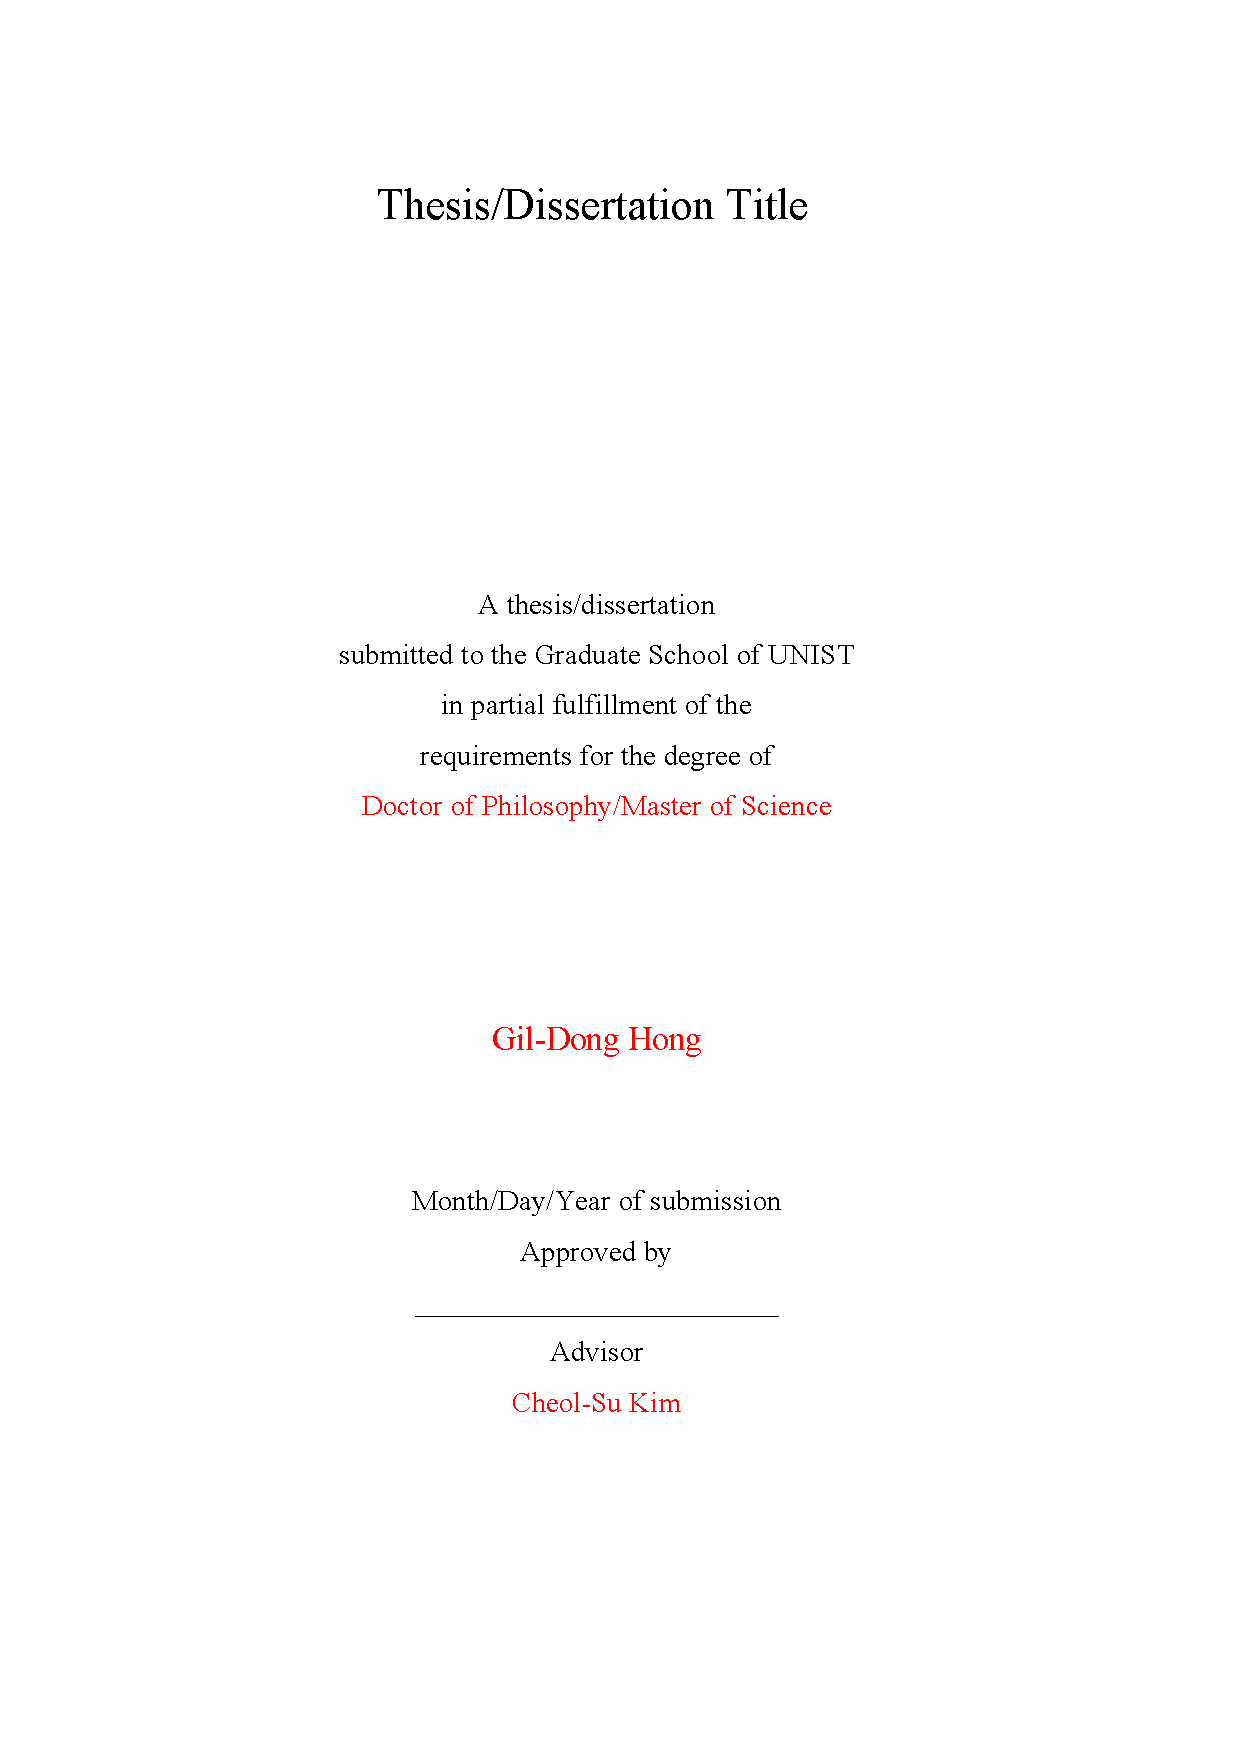
\includepdf[fitpaper= true, pages=-]{figures/cover/3.pdf}
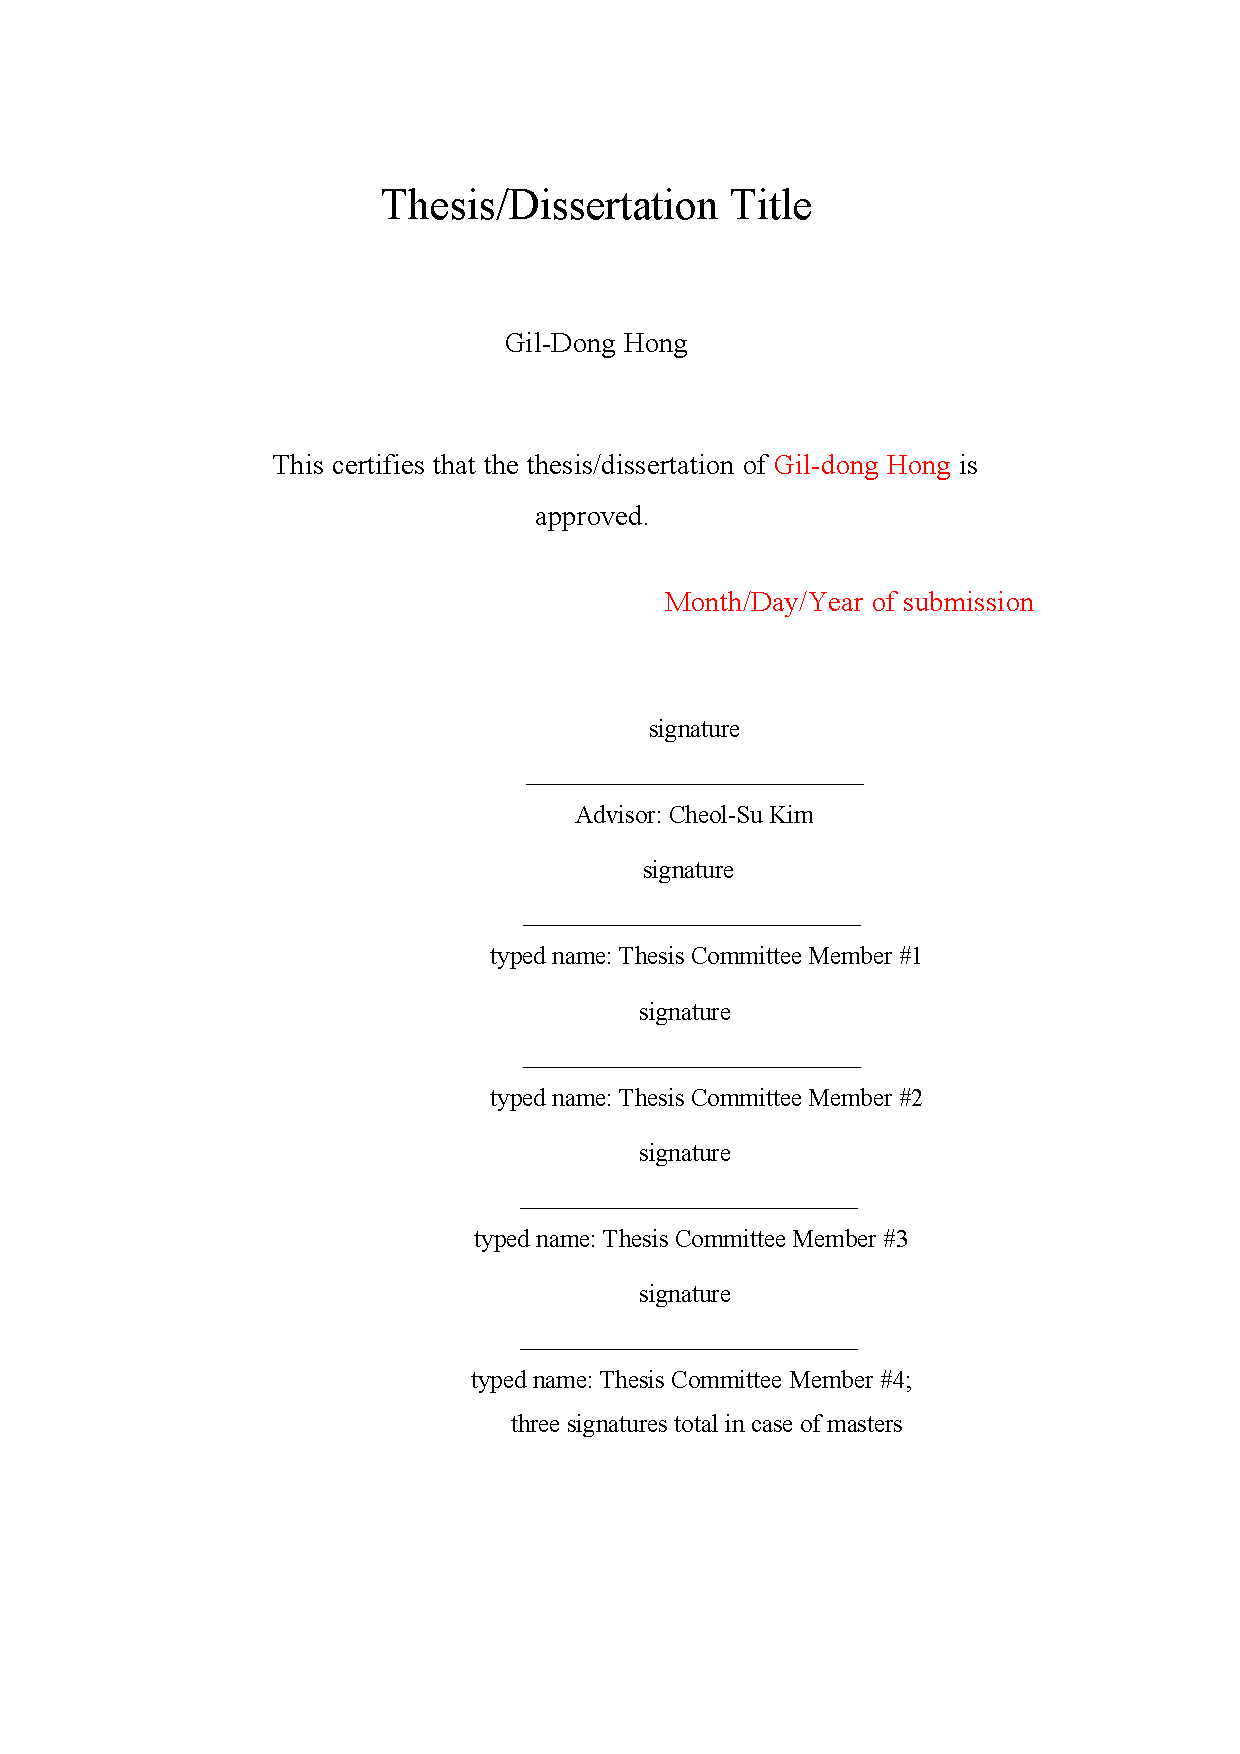
\includepdf[fitpaper= true, pages=-]{figures/cover/4.pdf}

% Abstract
\begin{abstract}
Your abstract should be here. \vfill
\end{abstract}

\clearpage


%%%%%%%%%%%%%%%%%%%%%%%%%%%%%%%%%%%%%%%%%%%%%%%%%%%%%%%%%%%%% 
%%%%%%%%%%    Do not touch the below 20 lines 
%%%%%%%%%%%%%%%%%%%%%%%%%%%%%%%%%%%%%%%%%%%%%%%%%%%%%%%%%%%%% 
%%% The following page is intentionally left as blank
%%% White attachment form
\hbox{ }
\thispagestyle{empty}
\clearpage

%%% Table of Contents
% \setcounter{page}{5}
\addcontentsline{toc}{section}{Table of Contents}
\tableofcontents{}
% \thispagestyle{empty}
% \vfill
\clearpage

%%% List of Figures
\addcontentsline{toc}{section}{List of Figures}
\listoffigures{}
% \thispagestyle{empty}
% \vfill
\clearpage

%%% List of Tables
\addcontentsline{toc}{section}{List of Tables}
\listoftables{}
% \thispagestyle{empty}
% \vfill
\clearpage

\begin{publications}
\noindent
This dissertation is based on the following publications.
\\\\
Lists
\\\\
Who did what for each publication

\end{publications}
\clearpage
%%%%%%%%%%%%%%%%%%%%%%%%%%%%%%%%%%%%%%%%%%%%%%%%%%%%%%%%%%%%% 
%%%%%%%%%%    Do not touch the above 20 lines 
%%%%%%%%%%%%%%%%%%%%%%%%%%%%%%%%%%%%%%%%%%%%%%%%%%%%%%%%%%%%% 

%%% reset page numbering
\pagenumbering{arabic}
\setcounter{page}{1}

%%%%%%%%%%%%%%%%%%%%%%%%%%%%%%%%%%%%%%%%%%%%%
% The sections will be shown in below order
%
% You can add/delete/modify the files in this folder
% 
% If you did, you should change here too.
%
% Abstract is already in the main.tex 
%%%%%%%%%%%%%%%%%%%%%%%%%%%%%%%%%%%%%%%%%%%%%

\section{Introduction}

Intro

\newpage
\section{Related Work}

RW

\newpage
\section{Chapter3:}

\subsection{Abstract}
test1
\subsubsection{Sub-contents}
test2
\paragraph{bullets}
test3

\newpage
\section{Chapter4:} 

Chapter4

\newpage 
\section{Chapter5}

Chapter5

\newpage
\section{Conclusion}

Conclusion

\clearpage

%%%%%%%%%%%%%%%%%%%%%%%%%%%%%%%%%%%%%%%%%%%%%
%			Reference
%%%%%%%%%%%%%%%%%%%%%%%%%%%%%%%%%%%%%%%%%%%%%
\citestyle{acmauthoryear}
% \citestyle{acmnumeric}
\addcontentsline{toc}{section}{References}
\bibliographystyle{unsrtnat}

\bibliography{references.bib}
\clearpage

%%%%%%%%%%%%%%%%%%%%%%%%%%%%%%%%%%%%%%%%%%%%%
%			Acknowledgment
%%%%%%%%%%%%%%%%%%%%%%%%%%%%%%%%%%%%%%%%%%%%%
\addcontentsline{toc}{section}{Acknowledgements}
\section*{\hfill \Large Acknowledgements \hfill}
Thank you very much.
\clearpage

%%%%%%%%%%%%%%%%%%%%%%%%%%%%%%%%%%%%%%%%%%%%%%%%%%%%%%%%%%%%% 
%%%%%%%%%%    Do not touch the below 
%%%%%%%%%%%%%%%%%%%%%%%%%%%%%%%%%%%%%%%%%%%%%%%%%%%%%%%%%%%%% 

%%% The following page is intentionally left as blank
% White attachment form
\hbox{ }
\thispagestyle{empty}
\clearpage

\end{document}